\subsection{Visualizzazione LLM salvati}

\begin{figure}[H]
    \centering
    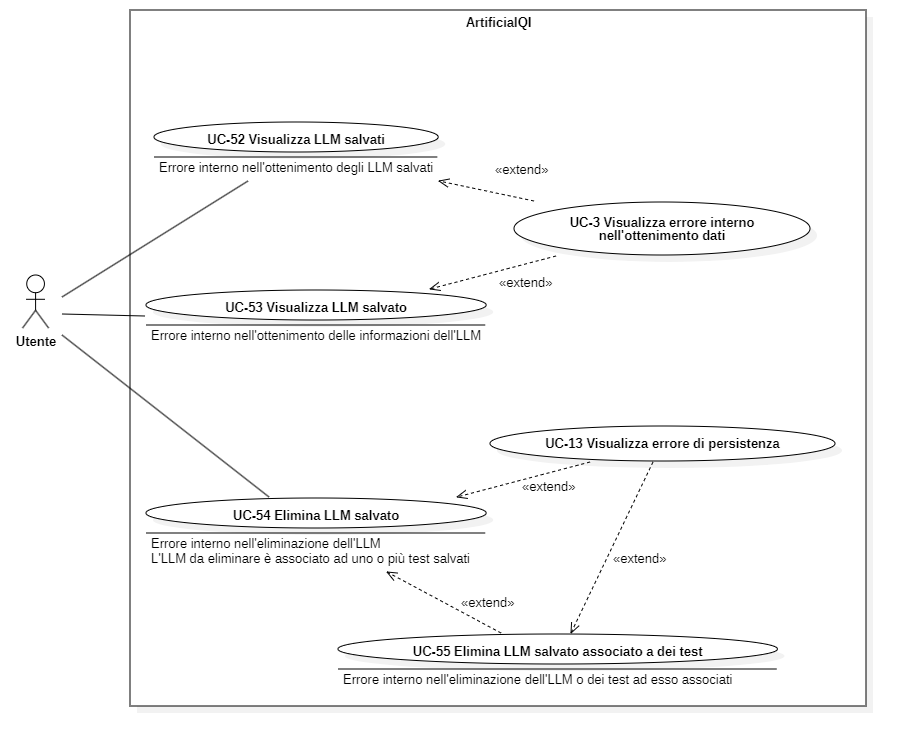
\includegraphics[scale=0.2]{Sezioni/UseCase/Immagini/VisualizzazioneLLMSalvati.png}
    \caption{Diagramma modifica dataset salvati.}
\end{figure}

\begin{usecase}{UC-55}{Visualizza LLM salvati}
    \label{uc:UC-55}
    
    \req{\hyperref[ru:RUF-6]{RUF-6}} 

    \pre{}

    \post{
        \item L'utente visualizza la lista degli LLM salvati
    }
    
    \actor{Utente}

    \trigger{L'utente vuole visualizzare la lista degli LLM salvati}

    \inc{}

    \base{}

    \scenario{
        \item L'utente richiede la visualizzazione degli LLM salvati
        \item Il sistema ottiene l'insieme di LLM salvati
        \item Il sistema verifica la presenza di LLM salvati       
        \item Il sistema mostra gli LLM salvati
    }

    \subscenario{
        \item[2.1] Avviene un errore interno al sistema durante l'ottenimento degli LLM salvati:
        \begin{itemize}
            \item \hyperref[uc:UC-3]{UC-3}
        \end{itemize}
        \item[3.1] Non esistono LLM salvati:
        \begin{itemize}
            \item Il sistema indica all'utente che non esistono ancora LLM salvati
        \end{itemize}
    }
\end{usecase}

\begin{usecase}{UC-56}{Visualizza LLM salvato}
    \label{uc:UC-56}
    
    \req{\hyperref[ru:RUF-6]{RUF-6}} 

    \pre{
        \item L'LLM da visualizzare esiste
        \item L'utente sta visualizzando gli LLM salvati \hyperref[uc:UC-55]{UC-55}
    }

    \post{
        \item L'utente visualizza le informazioni dell'LLM salvato
    }
    
    \actor{Utente}

    \trigger{L'utente vuole visualizzare le informazioni di un LLM salvato}

    \inc{}

    \base{}

    \scenario{
        \item L'utente richiede di visualizzare un LLM salvato
        \item Il sistema ottiene le informazioni sull'LLM       
        \item Il sistema mostra il nome e la configurazione per l'LLM
    }

    \subscenario{
        \item[2.1] Avviene un errore interno al sistema durante l'ottenimento delle informazioni sull'LLM:
        \begin{itemize}
            \item \hyperref[uc:UC-3]{UC-3}
        \end{itemize}
    }
\end{usecase}

\begin{usecase}{UC-57}{Elimina un LLM salvato}
    \label{uc:UC-57}
    
    \req{\hyperref[ru:RUF-6]{RUF-6}} 

    \pre{
        \item L'LLM da eliminare esiste
        \item L'utente sta visualizzando gli LLM salvati \hyperref[uc:UC-55]{UC-55}
    }

    \post{
        \item L'LLM viene eliminato
    }
    
    \actor{Utente}

    \trigger{L'utente vuole eliminare un LLM salvato}

    \inc{}

    \base{}

    \scenario{
        \item L'utente richiede l'eliminazione dell'LLM salvato
        \item Il sistema verifica che l'LLM non sia associato a test salvati 
        \item L'utente conferma l'eliminazione dell'LLM
        \item Il sistema elimina l'LLM
        \item Il sistema avvisa l'utente che l'eliminazione è avvenuta con successo
    }

    \subscenario{
        \item[2.1] L'LLM da eliminare è associato a uno o più test salvati:
        \begin{itemize}
            \item \hyperref[uc:UC-58]{UC-58}
        \end{itemize}
        \item[3.1] L'utente annulla l'eliminazione:
        \begin{itemize}
            \item Il sistema annulla l'operazione
        \end{itemize}
        \item[4.1] Avviene un errore interno al sistema durante l'eliminazione dell'LLM:
        \begin{itemize}
            \item \hyperref[uc:UC-16]{UC-16}
        \end{itemize}
    }
\end{usecase}

\begin{usecase}{UC-58}{Elimina LLM salvato associato a dei test}
    \label{uc:UC-58}
    
    \req{} 

    \pre{
        \item L'LLM da eliminare è associato a uno o  più test salvati
    }

    \post{
        \item L'LLM e i test a esso associati vengono eliminati dal sistema
    }
    
    \actor{}

    \trigger{Il sistema deve eliminare un LLM associato a uno o più test salvati}

    \inc{}

    \base{}

    \scenario{
        \item Il sistema visualizza la lista di test associati all'LLM e avvisa l'utente che verranno eliminati
        \item L'utente conferma l'eliminazione
        \item Il sistema elimina l'LLM 
        \item Il sistema elimina i test associati
        \item Il sistema avvisa l'utente della corretta eliminazione
    }

    \subscenario{
        \item[2.1] L'utente annulla l'operazione di eliminazione:
        \begin{itemize}
            \item Il sistema annulla l'operazione
        \end{itemize} 
        \item[3.1] Avviene un errore interno al sistema durante l'eliminazione dell'LLM:
        \begin{itemize}
            \item \hyperref[uc:UC-16]{UC-16}
        \end{itemize}
        \item[4.1] Avviene un errore interno al sistema durante l'eliminazione dei test associati:
        \begin{itemize}
            \item \hyperref[uc:UC-16]{UC-16}
        \end{itemize}
    }
\end{usecase}